\chapter{Virtual memory}
\emph{Virtual memory} provides a separation of user logical memory from physical memory. Only part of the program needs to be in memory for execution, therefore logical address space can be much larger than physical address space. Virtual memory allows address spaces to be shared by several processes and it allows a more efficient process creation. It can be implemented via demand paging or demand segmentation.

\section{Demand paging}
\emph{Demand paging} consists of bringing a page into memory only when it is needed, leading to less input/output operations, less memory needed and faster response. An invalid reference causes an abort, while a not-in-memory fault causes a page fault exception.

Demand paging works because of the locality model. In fact, process migrates from one locality to another. These localities may overlap.

With each entry in the page table, a valid-invalid bit is associated, initially set to invalid (i.e.,\@ not-in memory) on all entries. During address translation, if valid-invalid bit in page table entry is set to invalid, a page fault occurs.

A swapper that deals with pages is a \textbf{pager}.

\paragraph{Page fault}
If there is a reference to a page, first reference to that page will trap the operating system: \emph{page fault}.
\begin{enumerate}
\item Operating system looks at another table to decide:
\begin{itemize}
\item Invalid reference $\Rightarrow$ abort;
\item Just not in memory;
\end{itemize}
\item Get empty frame;
\item Swap page into frame;
\item Reset tables;
\item Set validation bit;
\item Restart the instruction that caused the page fault.
\end{enumerate}

\begin{figure}[hbtp]
\centering
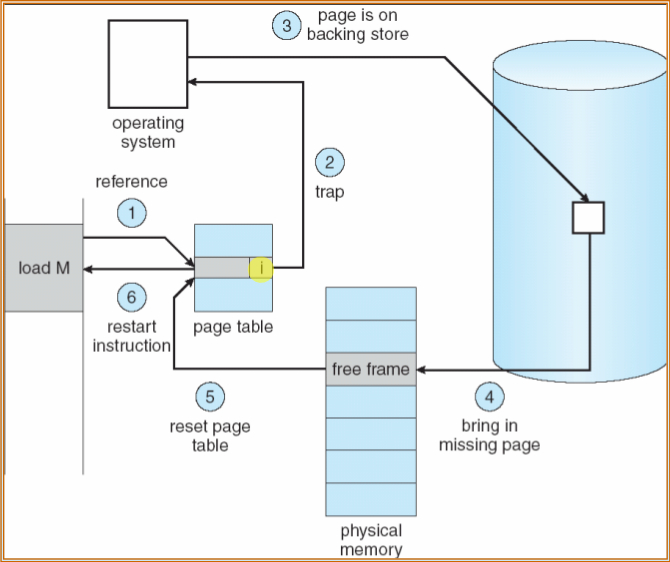
\includegraphics[scale=0.4]{images/virtual_memory/page_fault.jpg}
\caption{Page fault handling}
\end{figure}

$\text{EAT} = (1-p) t_{memory} + p (t_{page\ fault} + t_{swap\ out} + t_{swap\ in} + t_{restart})$ being $ 0 \le p \le 1 $, page fault ratio.

\subsection{Page replacement}
If there is no free frame, it is needed to find some page in memory not really in use and swap it out.
\begin{itemize}
\item Prevent over-allocation of memory by modifying page-fault service routine to include page replacement;
\item Use modify (dirty) bit to reduce overhead of page transfers: only modified pages are written to disk;
\item Page replacement completes separation between logical and physical memory. Larger virtual memory can be provided on a smaller physical memory.
\end{itemize}

\paragraph{Basic algorithm}
\begin{enumerate}
\item Find the location of the desired page on disk;
\item Find a free frame:
\begin{itemize}
\item If there is a free frame, use it;
\item If there is no free frame, use a page replacement algorithm to select a victim frame;
\end{itemize}
\item Bring the desired page into the newly free frame and update page and frame tables;
\item Restart the process.
\end{enumerate}

\paragraph{Optimal Algorithm}
Replace page that will not be used for longest period of time. Used for measuring every algorithm performance. It is unfeasible because it should predict the future.

\paragraph{FIFO Algorithm}
\begin{center}
\begin{tabular}{l|cccccccccccc}
\hline
Time & 1 & 2 & 3 & 4 & 5 & 6 & 7 & 8 & 9 & 10 & 11 & 12 \\
\hline
String & 4 & 3 & 2 & 1 & 4 & 3 & 5 & 4 & 3 & 2 & 1 & 5 \\
\hline
Fault & • & • & • & • & • & • & • &  &  & • & • &  \\
\hline
Frame 1 & 4 & 3 & 2 & 1 & 4 & 3 & 5 & 5 & 5 & 2 & 1 & 1 \\
Frame 2 & & 4 & 3 & 2 & 1 & 4 & 3 & 3 & 3 & 5 & 2 & 2 \\
Frame 3 &  &  & \textbf{4} & \textbf{3} & \textbf{2} & \textbf{1} & 4 & 4 & \textbf{4} & \textbf{3} & 5 & 5 \\
\hline
\end{tabular}
\[ f = 10/12 = 83 \% \]
\end{center}
This algorithm is subjected to Belady's Anomaly: adding more frames will cause more page faults.

\begin{figure}[hbtp]
\centering
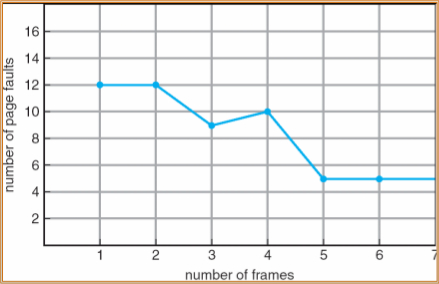
\includegraphics[scale=0.4]{images/virtual_memory/belady_anomaly.jpg}
\caption{Belady's Anomaly}
\end{figure}

\paragraph{Least Recently Used Algorithm}
Every page entry has a counter; every time page is referenced through this entry, the clock is copied into the counter. When a page needs to be changed, look at the counters to determine which are to change.

\begin{center}
\begin{tabular}{l|cccccccccccc}
\hline
Time & 1 & 2 & 3 & 4 & 5 & 6 & 7 & 8 & 9 & 10 & 11 & 12 \\
\hline
String & 4 & 3 & 2 & 1 & 4 & 3 & 5 & 4 & 3 & 2 & 1 & 5 \\
\hline
Fault & • & • & • & • & & & • & & & • & • & • \\
\hline
Frame 1 & 4 & 3 & 2 & 1 & 4 & 3 & 5 & 4 & 3 & 2 & 1 & 5 \\
Frame 2 & & 4 & 3 & 2 & 1 & 4 & 3 & 5 & 4 & 3 & 2 & 1 \\
Frame 3 & & & \textbf{4} & \textbf{3} & \textbf{2} & \textbf{1} & 4 & 3 & \textbf{5} & \textbf{4} & 3 & 2 \\
\hline
\end{tabular}
\[ f = 10/12 = 83 \% \]
\end{center}

A possible implementation is the \textbf{stack implementation} which keeps a stack of page numbers in a double link form:
\begin{itemize}
\item Page referenced
\begin{itemize}
\item Move it to the top;
\item Requires six pointers to be changed;
\end{itemize}
\item No search for replacement.
\end{itemize}
This implementation causes a large overhead and therefore is unfeasible and not used in reality.

\subparagraph{Least Recently Used Stack}
Adding a new page cannot increase the number of page faults. In fact, the old ``stack'' is the same and it can keep a new page.
\begin{center}
\begin{tabular}{l|cccccccccccc}
\hline
Time & 1 & 2 & 3 & 4 & 5 & 6 & 7 & 8 & 9 & 10 & 11 & 12 \\
\hline
String & 4 & 3 & 2 & 1 & 4 & 3 & 5 & 4 & 3 & 2 & 1 & 5 \\
\hline
Fault & • & • & • & • & • & • & • & & & • & • & • \\
\hline
Frame 1 & 4 & 3 & 2 & 1 & 4 & 3 & 5 & 4 & 3 & 2 & 1 & 5 \\
Frame 2 & & 4 & 3 & 2 & 1 & 4 & 3 & 5 & 4 & 3 & 2 & 1 \\
Frame 3 & & & 4 & 3 & 2 & 1 & 4 & 3 & 5 & 4 & 3 & 2 \\
Frame 4 & & & & 4 & 3 & \textbf{2} & 1 & 1 & \textbf{1} & \textbf{5} & \textbf{4} & 3 \\
\hline
\end{tabular}
\[ f = 8/12 = 75 \% \]
\end{center}

\paragraph{LRU Approximation Algorithms}
\subparagraph{Reference bit}
Select a page which has not been referred for a certain amount of time, i.e.,\@ since the last page fault.
\begin{itemize}
\item With each page associate a bit, initially set to zero;
\item When page is referenced bit is set to 1;
\item Replace the page where bit is 0, if one exists.
\end{itemize}
\subparagraph{Second chance}
\begin{itemize}
\item Need reference bit;
\item Clock replacement;
\item If page to be replaced (in clock order) has reference bit set to 1, then:
\begin{itemize}
\item Set reference bit to 0;
\item Leave page in memory;
\item Replace next page in clock order, subject to same rules.
\end{itemize}
\end{itemize}

\subsection{Allocation of frames}
Each process needs \emph{minimum} number of pages. Two major allocation schemes:
\begin{description}
\item [Fixed allocation] Allocation can be equal (i.e.,\@ assign an equal number of frames among processes) or proportional (i.e.,\@ assign a number of frames according to the size of process).
\item [Priority allocation] Use a proportional allocation scheme using priority numbers rather than size. If a process generates a page fault, select for replacement one of its frames or select for replacement a frame from a process with lower priority number.
\end{description}
Two strategies are possible for page replacement:
\begin{description}
\item [Global replacement] Each process selects a replacement frame from the set of all frames; one process can take a frame from another.
\item [Local replacement] Each process selects from only its own set of allocated frames.
\end{description}
If a process does not have ``enough'' pages, page-fault rate is very high, leading to low CPU utilization which makes the operating system thinking that it needs to increase the degree of multiprogramming, therefore a new process is added which cause an even lower CPU utilization.

\textbf{Thrashing} means that a process is busy swapping pages in and out.

\begin{figure}[hbtp]
\centering
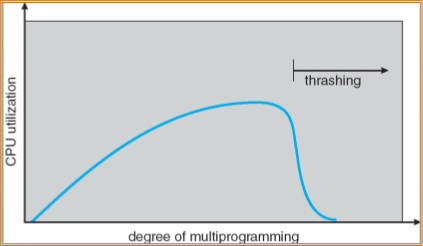
\includegraphics[scale=0.4]{images/virtual_memory/thrashing.jpg}
\caption{Thrashing}
\end{figure}

\subsection{Working-Set Model}
Defining $\Delta$ as the working-set windows (i.e.,\@ a fixed number of page references), it is possible to define ${WSS}_i$ as the working set of process $P_{i}$ (i.e.,\@ the total number of pages referenced in the most recent $\Delta$).
\begin{itemize}
\item If $\Delta$ is too small, it will not encompass entire locality;
\item If $\Delta$ is too large, it will encompass several localities;
\item If $\Delta = \infty$, it will encompass entire program.
\end{itemize}
The working-set strategy has a variable \emph{resident set}, $\overline{RT} = \dfrac{1}{T} \sum_{t=1}^T RS(t,\Delta)$.

\subsection{Page-Fault Frequency Scheme}
It is needed to establish ``acceptable'' page-fault rate ($1/c$ where $c$ is the time between two page faults). If actual rate is too low, the process loses frame. On the other hand, if actual rate is too high, process gains frame.

\paragraph{Strategy}
Run at each page fault, not at every reference. It is controlled by the time interval between page faults.
\begin{itemize}
\item If $\tau < c$, i.e.,\@ the measured page fault frequency is greater than the one acceptable, a page has to e added to the Resident Set of the process issuing this page fault;
\item If $\tau > c$, all pages not referred in that interval by the current process are eliminated from its Resident Set. The reference bit of all pages in the Resident Set are cleared.
\end{itemize}

\begin{figure}[hbtp]
\centering
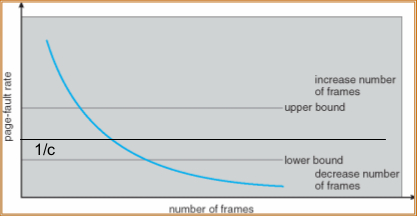
\includegraphics[scale=0.6]{images/virtual_memory/page_fault_frequency.jpg}
\caption{Page-Fault frequency scheme}
\end{figure}

\subsection{Other issues}
\paragraph{Prepaging}
To reduce the large number of page faults that occurs at process startup, prepage all or some of the pages a process will need, before they are referenced but if prepaged pages are unused, I/O and memory was wasted.

Assuming $s$ pages are prepaged and $\alpha$ of the pages is used, it is needed to compare the cost of $s \cdot \alpha$ save pages faults with the cost of prepaging $s \cdot (1-\alpha)$ unnecessary pages.

\paragraph{Page size}
Page size selection must take into consideration fragmentation, table size, I/O overhead and locality.